\chapter{Energy}

\section*{Level of clean energy capacity (megawatts) installed as a result of International Climate Finance (ICF) support.}

\thispagestyle{empty}


\section{Results}

From 2015/16 to 2019/20 DFID installed \textbf{771 megawatts} of clean energy capacity (Table \ref{tab:energy}). %

\begin{figure}[htbp]
	\centering
	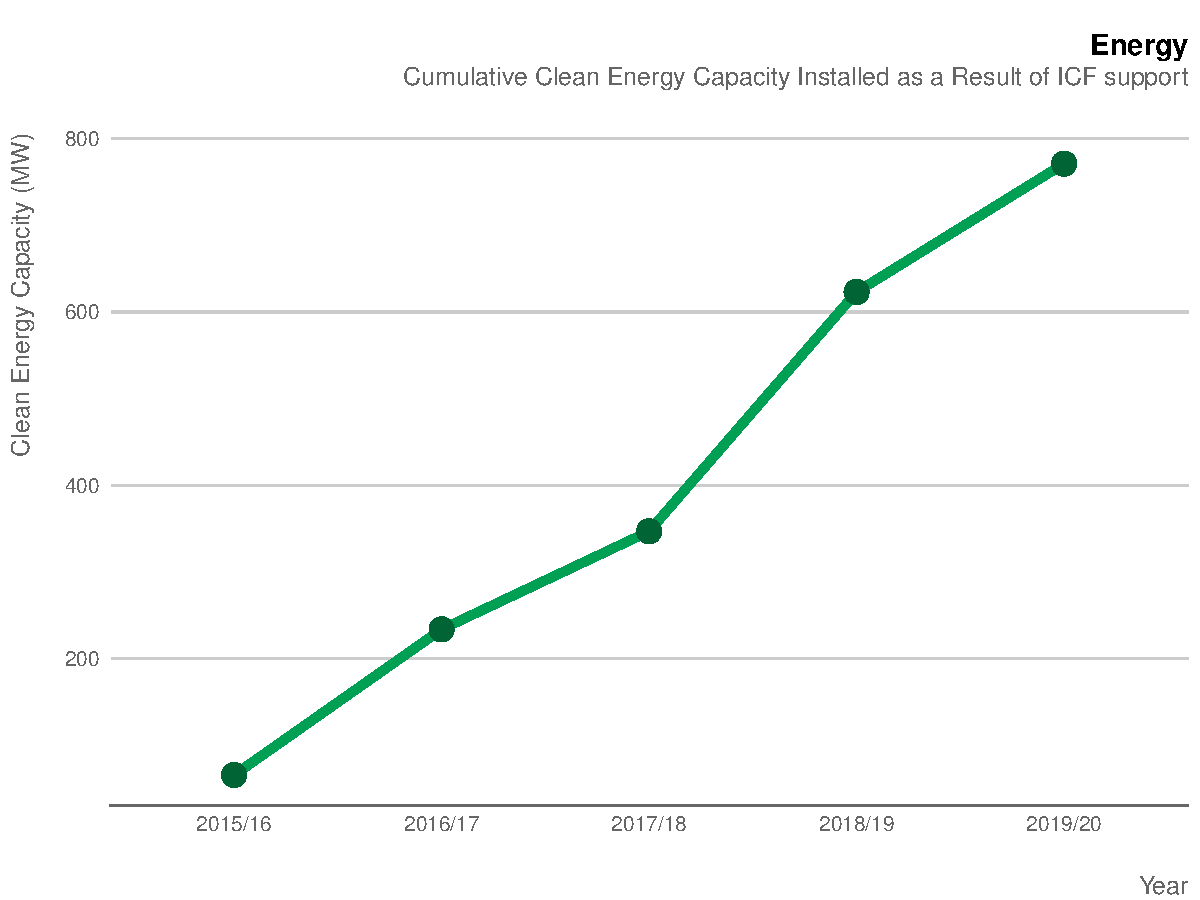
\includegraphics[width=0.7\textwidth]{../figs/energy_cumulative_plot} \hfill
	\caption{Line plot of cumulative clean energy capacity installed (in megawatts) from 2015/16 to 2019/20.}
	\label{fig:energy_cumulative_plot}
\end{figure}

Historical annual estimates are updated during each new results reporting round to reflect the best available information on programme achievements. %
As a result, several corrections to past years' data from the Clean Technology Fund (CTF), were made following a review of Climate Investment Funds (CIF) results by relevant inputting Multilateral Development Banks (MDB) and the CIFs Audit Unit. %
Corrections have been made where it was discovered that either results were being taken from the wrong source, data were input incorrectly, or inappropriate adjustments for over/under reporting had been made. %
This year, a portion of the private finance leveraged by some projects has been reclassified as coming from public sources, causing a fall in private finance leveraged while also driving an increase in public finance leveraged.  %
These errors are difficult to catch during the quality assurance process as the CIFs rely on the relevant managing MDBs to report project data accurately in the first instance. %

\begin{table}[htbp]
	\centering
	\caption{Cumulative Totals of MW Clean Energy Capacity Installed (ICF KPI 7)}\label{tab:energy}
	\begin{tabular}{rrrrr}
		\toprule
		\multicolumn{1}{c}{\textbf{2015/16}}&\multicolumn{1}{c}{\textbf{2016/17}}&\multicolumn{1}{c}{\textbf{2017/18}}&\multicolumn{1}{c}{\textbf{2018/19}}&\multicolumn{1}{c}{\textbf{2019/20}} \\ \hline
		\rule{0pt}{10pt}66 	  &      234 	&        347 	   &     623 	  &        771 \\ \bottomrule
	\end{tabular}
\end{table}

\section{Context}

This indicator measures clean energy capacity installed as a result of DFID
programming. %

Access to energy is the number one constraint to inclusive economic growth and job creation. %
Over one billion people lack access to modern energy, 95\% of whom live in Africa and South Asia. %
Access to energy is a critical constraint to growth across all DFID’s focus countries, and lack of reliable power reduces African GDP by 2-4\%. %

Population growth is also pushing up energy demand; investments in electricity generation, transmission and distribution and connections have failed to keep pace. %
We are doing more to help meet businesses' rising energy needs; to ensure
affordable energy access for the poor; and to enhance environmental sustainability
in energy use. %
In our economic development strategy we made clear we will adopt a `climate smart' approach across our economic development work - including through sustainable energy. %


\newpage
